\documentclass{article}

\usepackage{graphicx}
\usepackage{tikz}
\usepackage{tikzsymbols}
\usetikzlibrary{calc,patterns,shapes.geometric}
\pagestyle{empty}
\usepackage[margin=0pt]{geometry}
\geometry{papersize={14in,12in}}

\def\centerarc[#1](#2)(#3:#4:#5){\draw[#1] ($(#2)+({#5*cos(#3)},{#5*sin(#3)})$) arc (#3:#4:#5);}

\begin{document}
	\begin{figure}
		\centering
		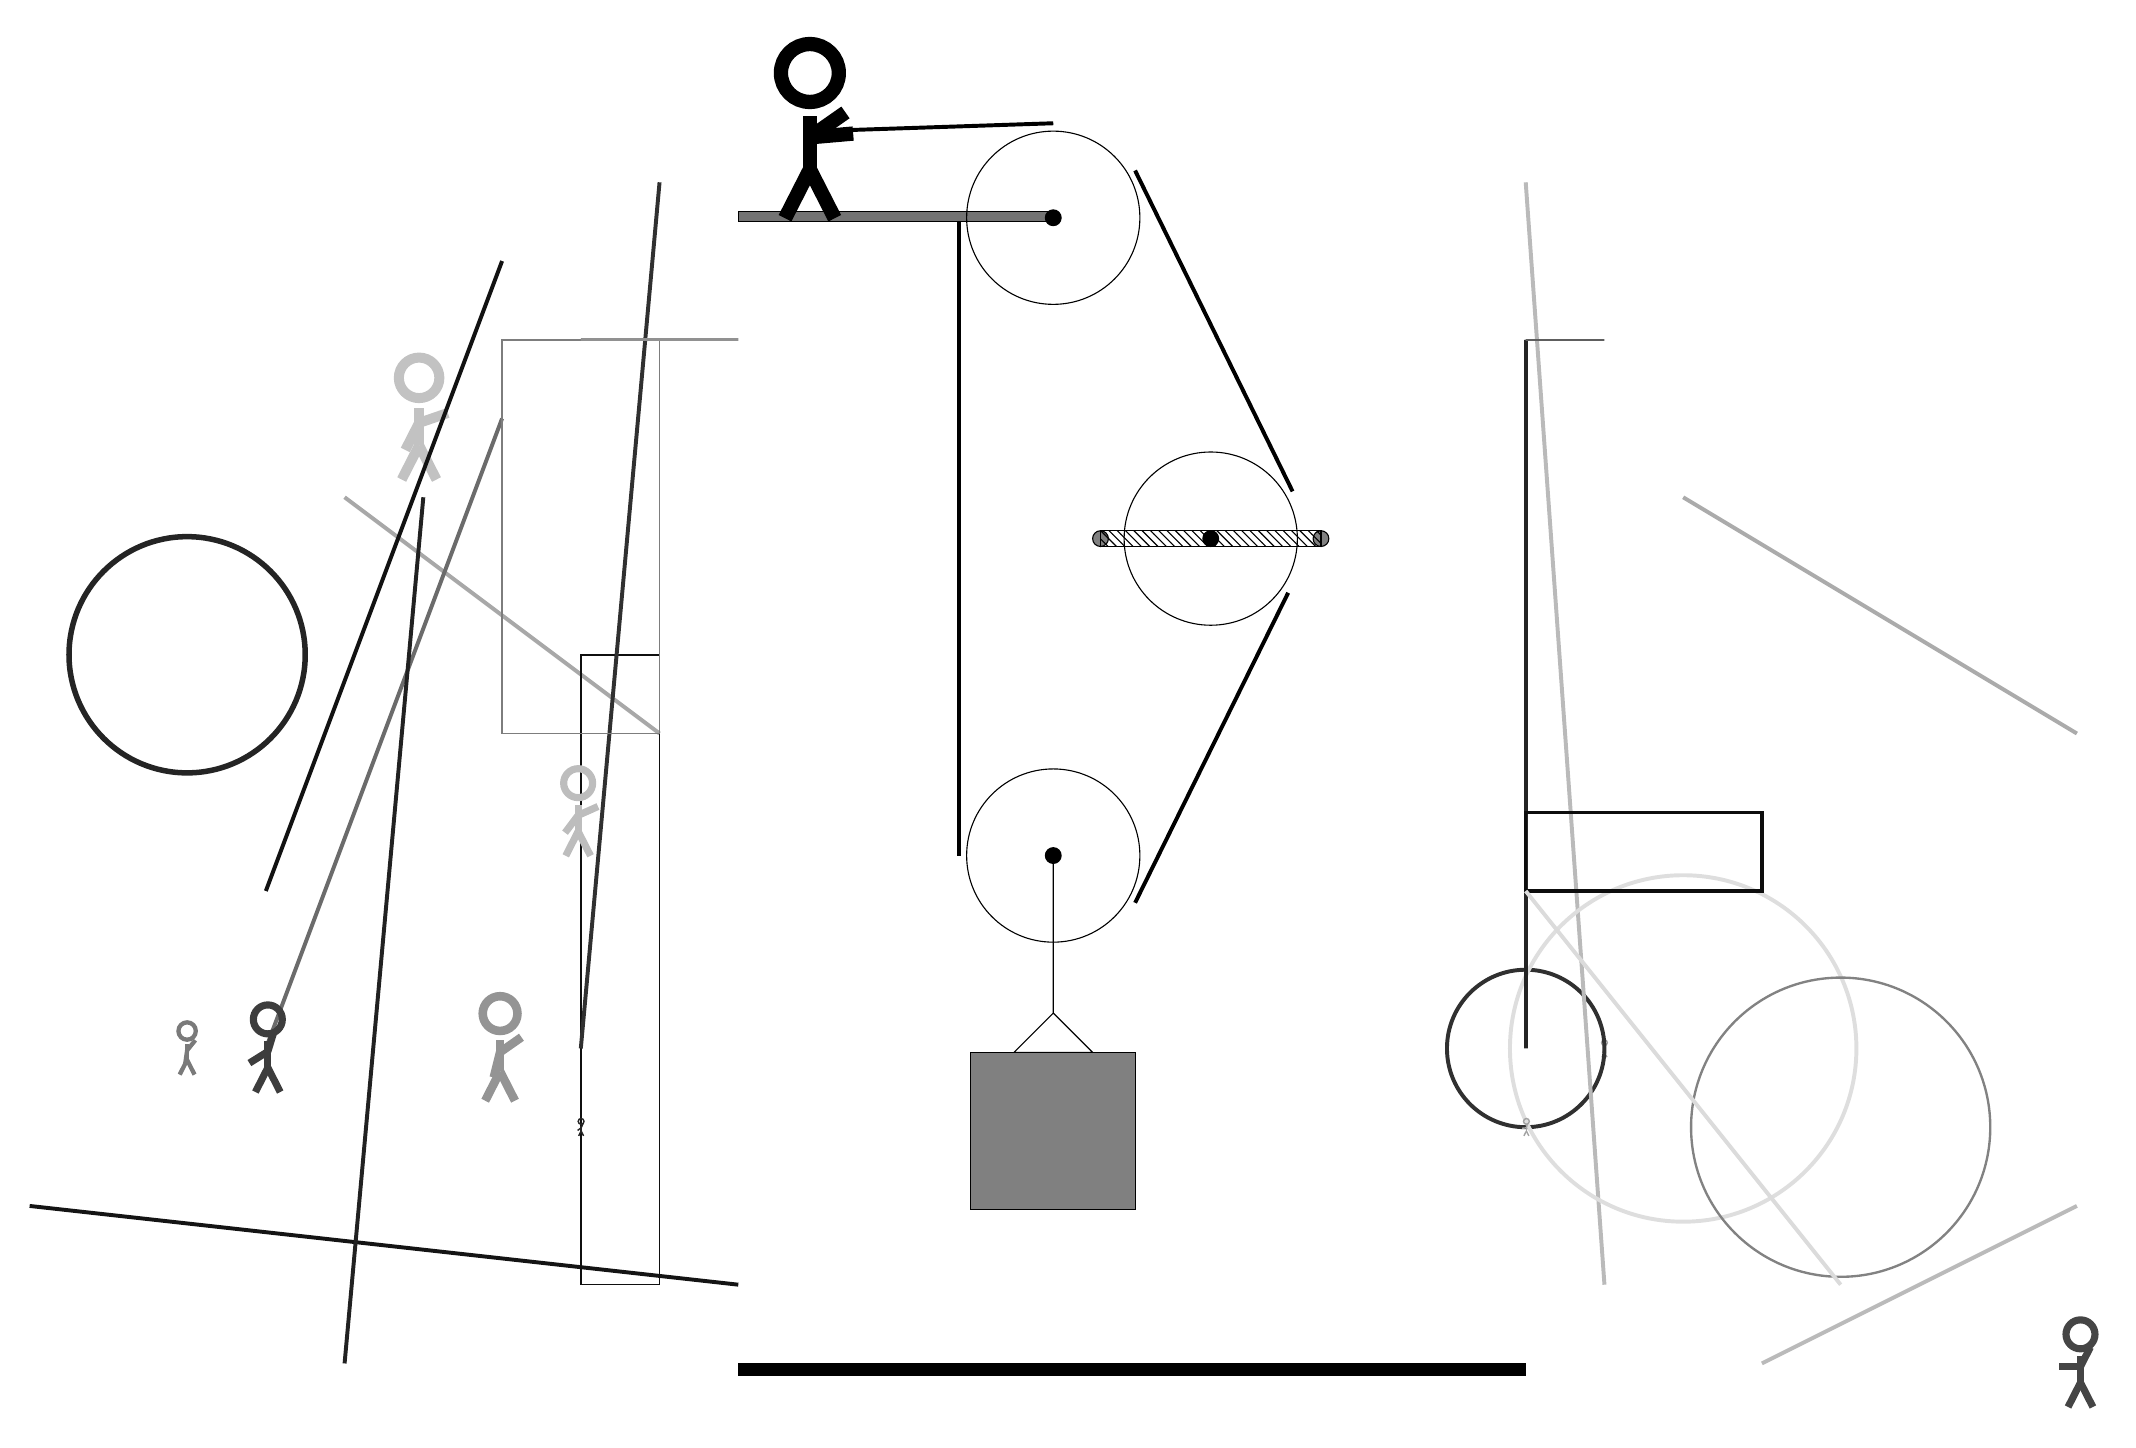
\begin{tikzpicture}
			%%%%% START %%%%%
			
			\draw[fill=black!55] (-2, 11.5) rectangle (2, 11.625);
			
			\draw (2, 3.45) circle (1.1);
			\draw[fill=black] (2, 3.45) circle (0.1);
			
			\draw (2, 11.55) circle (1.1);
			\draw[fill=black] (2, 11.55) circle (0.1);
			
			\draw[fill=white](4, 7.475) circle (1.1);
			\draw[fill=black] (4, 7.475) circle (0.1);
			\draw[fill=black!50] (2.6, 7.475) circle (0.1);
			\draw[fill=black!50] (5.4, 7.475) circle (0.1);
			\draw[pattern=north west lines, pattern color=black] (2.6, 7.575) rectangle (5.4, 7.375);
			
			\draw (2, 3.45) -- (2, 1.45) -- (1.5, 0.95) -- (2.5, 0.95) -- (2, 1.45);
			\draw[fill=black!50] (0.95, 0.95) rectangle (3.05, -1.05);
			
			\draw[line width=0.5mm] (0.8, 11.5) -- (0.8, 3.45);
			\centerarc[line width=0.5mm](2, 3.45)(180:330:1.2000000000000002);
			\draw[line width=0.5mm](3.0392, 2.85) -- (4.983, 6.7867);
			\centerarc[line width=0.5mm](4, 7.475)(390:325:1.2000000000000002);
			\draw[line width=0.5mm](5.0392, 8.075) -- (3.0392, 12.15);
			\centerarc[line width=0.5mm](2, 11.55)(30:90:1.2000000000000002);
			\draw[line width=0.5mm](2, 12.75) -- (-1, 12.65);
			
			\node[line width=0.3mm, color=black!37] at (9, 1) {\Strichmaxerl[1][63][77]};
			
			\draw[line width=0.5mm, color=black!27](11, -3) -- (15, -1);
			\draw [line width=0.5mm, color=black!81](8, 1) circle (1.0);
			\draw[line width=0.5mm, color=black!34](-3, 5) -- (-7, 8);
			\draw[line width=0.5mm, color=black!27](9, -2) -- (8, 12);
			
			\draw [line width=0.5mm, color=black!13](10, 1) circle (2.2);
			\draw[line width=0.5mm, color=black!92](-2, -2) -- (-11, -1);
			\draw[line width=0.5mm, color=black!86] (8, 10) rectangle (8, 1);
			\node[line width=0.6mm, color=black!42] at (-5, 1) {\Strichmaxerl[6][76][35]};
			\draw[line width=0.5mm, color=black!58](-5, 9) -- (-8, 1);
			
			\draw[line width=0.2mm, color=black!94] (-4, -2) rectangle (-3, 6);
			\draw[line width=0.5mm, color=black!87](-6, 8) -- (-7, -3);
			\draw[line width=0.5mm, color=black!81](-4, 1) -- (-3, 12);
			\draw [line width=0.3mm, color=black!49](12, 0) circle (1.9);
			\node[line width=0.3mm, color=black!86] at (-4, 0) {\Strichmaxerl[1][37][65]};
			\node[line width=0.2mm, color=black!36] at (8, 0) {\Strichmaxerl[1][6][77]};
			\node[line width=0.4mm, color=black!24] at (-6, 9) {\Strichmaxerl[7][63][19]};
			\draw[line width=0.2mm, color=black!51] (-3, 10) rectangle (-5, 5);
			\draw[line width=0.4mm, color=black!95] (8, 3) rectangle (11, 4);
			\draw[line width=0.5mm, color=black!14](12, -2) -- (8, 3);
			\node[line width=0.5mm, color=black!52] at (-9, 1) {\Strichmaxerl[3][82][51]};
			
			\draw[line width=0.3mm, color=black!63] (8, 10) rectangle (9, 10);
			\draw[line width=0.4mm, color=black!43] (-2, 10) rectangle (-4, 10);
			\node[line width=0.4mm, color=black!26] at (-4, 4) {\Strichmaxerl[5][53][24]};
			\draw [line width=0.7mm, color=black!86](-9, 6) circle (1.5);
			
			\node[line width=0.4mm, color=black!73] at (15, -3) {\Strichmaxerl[5][0][63]};
			\draw[line width=0.5mm, color=black!33](10, 8) -- (15, 5);
			\draw[line width=0.5mm, color=black!93](-5, 11) -- (-8, 3);
			\node[line width=0.5mm, color=black!76] at (-8, 1) {\Strichmaxerl[5][32][73]};
			
			\node at (-1, 12.65) {\Strichmaxerl[10][-175][35]};
			
			\draw[fill=black] (-2, -3) rectangle (8, -3.15);
			
			%%%%% END %%%%%
		\end{tikzpicture}
	\end{figure}	
\end{document}